\newpage
\section{Результати роботи}
Нижче ви можете бачити як вигдядає сайт на широкому дисплеї.

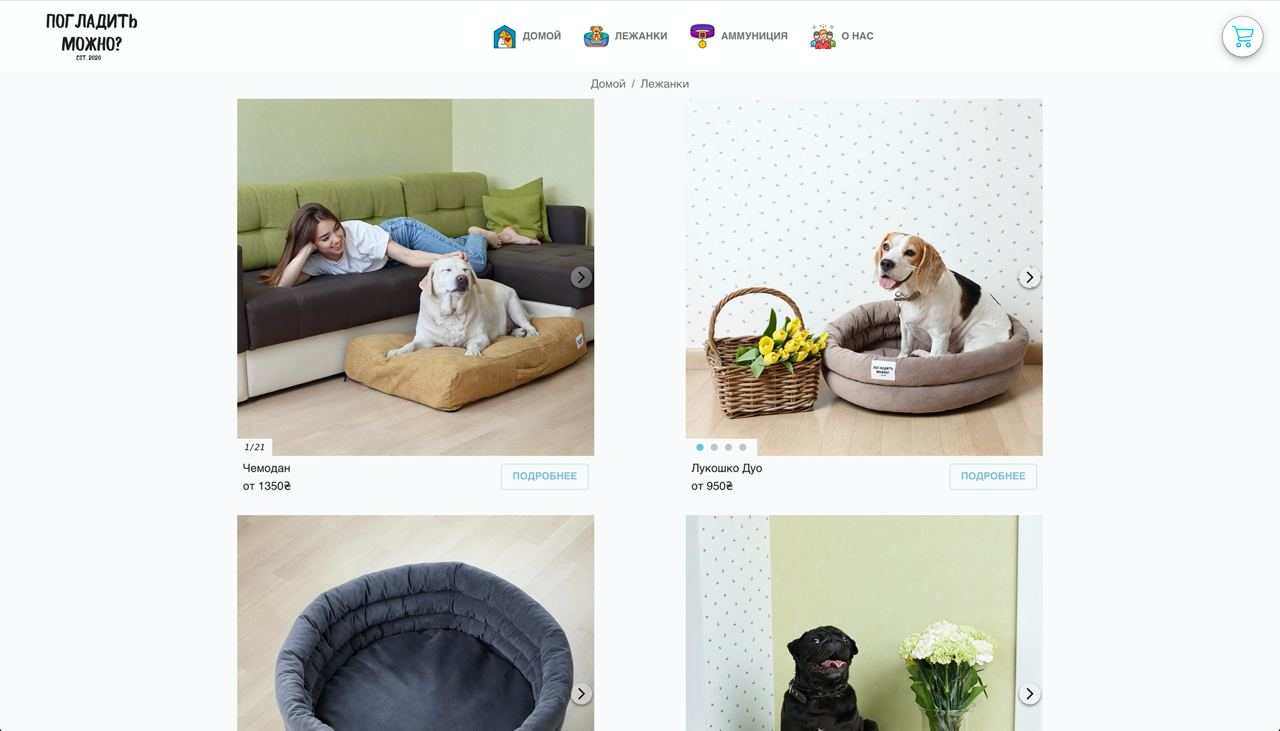
\includegraphics[width=0.9\textwidth]{../site_screenshot.jpg}

Далі продемонструємо результуюче значення метрик розглянутих в роботі.

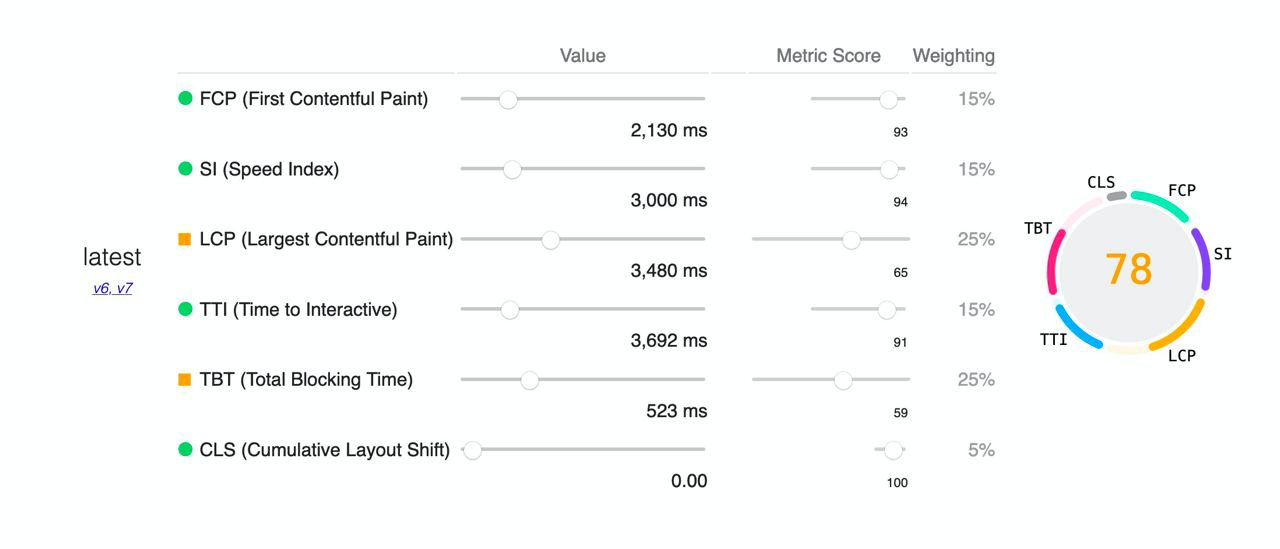
\includegraphics[width=0.9\textwidth]{../score.jpg}

На цьому зображенні ми можемо бачити результат з точки зору швидкості однієї зі сторінок сайту.
Ось цієї \\ https://pogladit-mozhno.vercel.app/categories/beds/products. \\
На ній знаходиться багато картинок це є основним фактором який уповільнює її.
Втім можемо бачити що за допомогою вище наведених методів вона працює дуже добре.

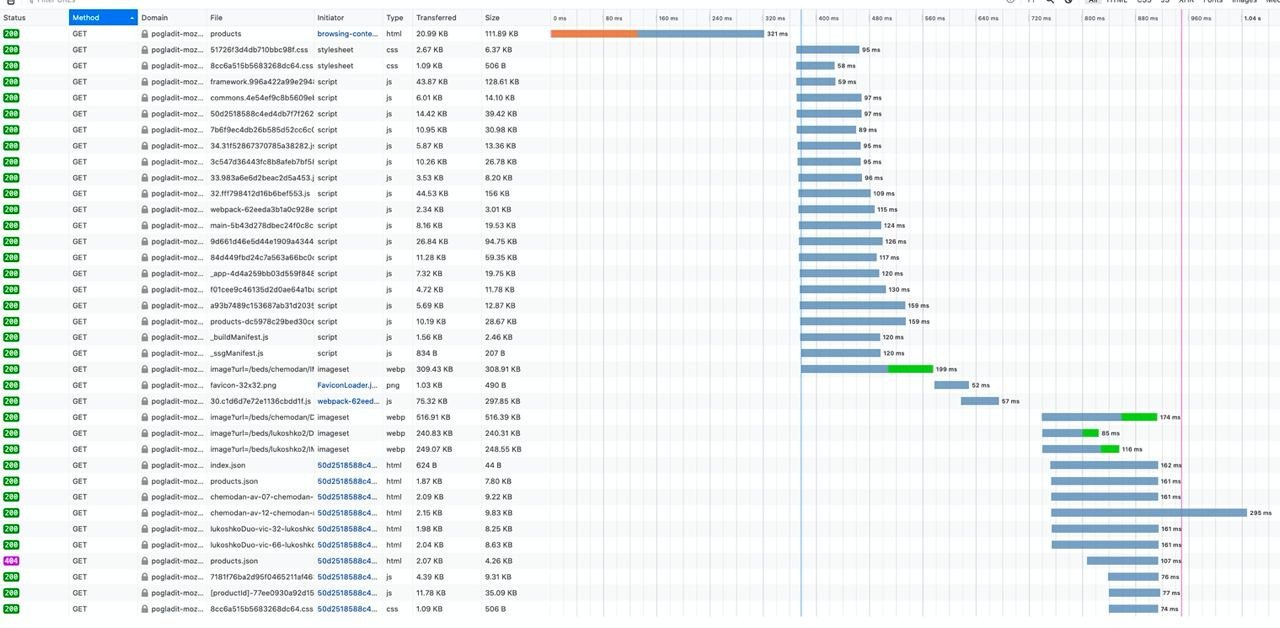
\includegraphics[width=0.8\textwidth]{../network_spec.jpg}


\begin{figure*}
    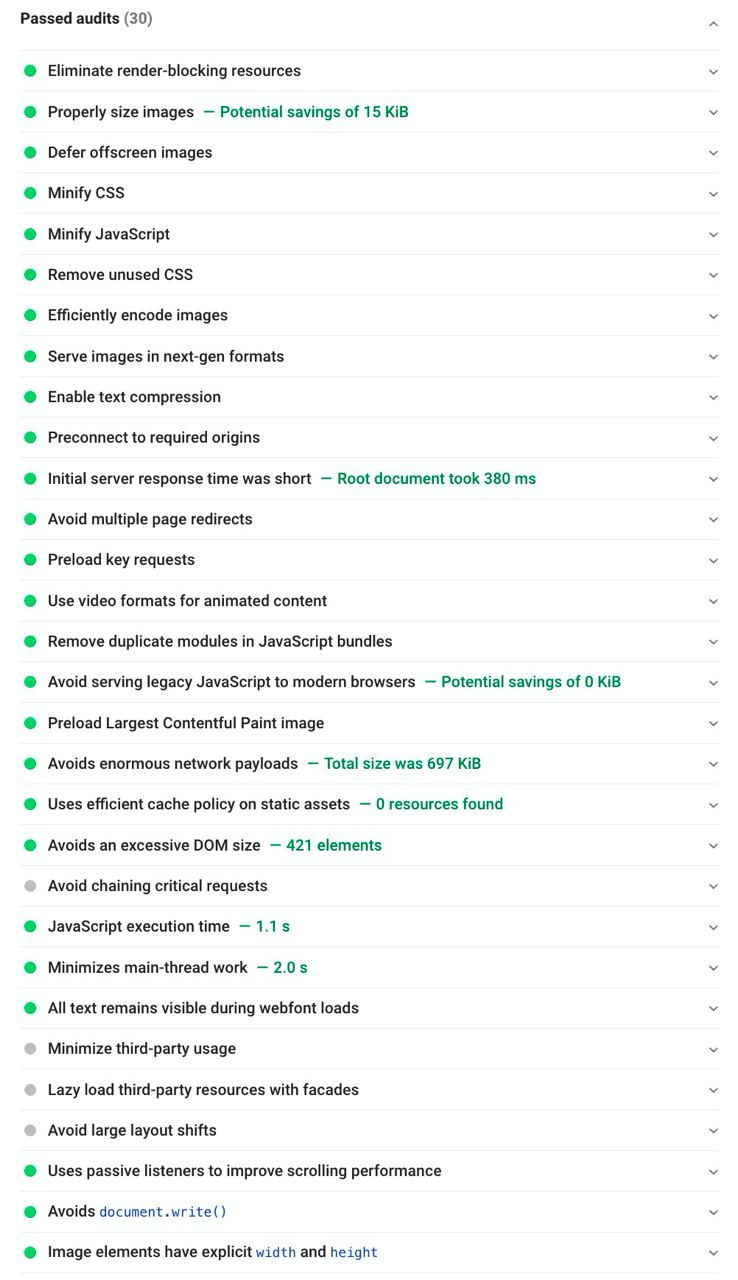
\includegraphics[width=0.8\linewidth]{../passed_audits.jpg}\par
    \caption{Пройдені тести.}
\end{figure*}

Вони демонструють якість сторінки та відповідність найкращим практикам.

На цьому зображенні видно як швидко загружається частини сторінки.
Серед двох зображень, які є на сторінці, перше (дивитись на формат webp) має вищий пріоритет та загружається
значно швидше через оптимізацію, яка була описана вище.
Далі можемо бачити що першим загружається HTML сторінка. Потім паралельно загружаються усі скрипти.
Наприкінці ми бачимо що сторінки загружаються наперед. Ця техніка була писала вище.
Для даного випадку вона є доволі ефективною.

\section{План розробки сайту}
У цій частині роботи я наведу приблизний план як можна розроблювати безплатний, швидкий, швидкий для розробки сайт.
Використовувати React та Next.
Почати з прикладу який більш за все схожий на задачу.
Наприклад для онлайн магазина https://github.com/vercel/commerce,
Для блогу шукати Next MDX. MDX є зручним та простим способом ведення сторінки.
Інші приклади може бути знайдені за адресою \\ https://github.com/vercel/next.js/tree/canary/examples

\begin{enumerate}
    \item Знайти приклад спланувати репозиторій.
    \item Розібратися з технологіями і дивлячись на код та роблячи маленькі зміни.
    \item Ітеративний наповнити сайт змістом.
    \item Згодом почати оптимізація швидкості сайту. Наприклад оптимізація картинок може відкладена на потім. Але наприклад про те що не потрібні бібліотеки краще не використовуватиТреба пам'ятати з початку.
\end{enumerate}
